\documentclass{standalone}
\usepackage{tikz}
\usetikzlibrary{patterns, positioning}

\begin{document}
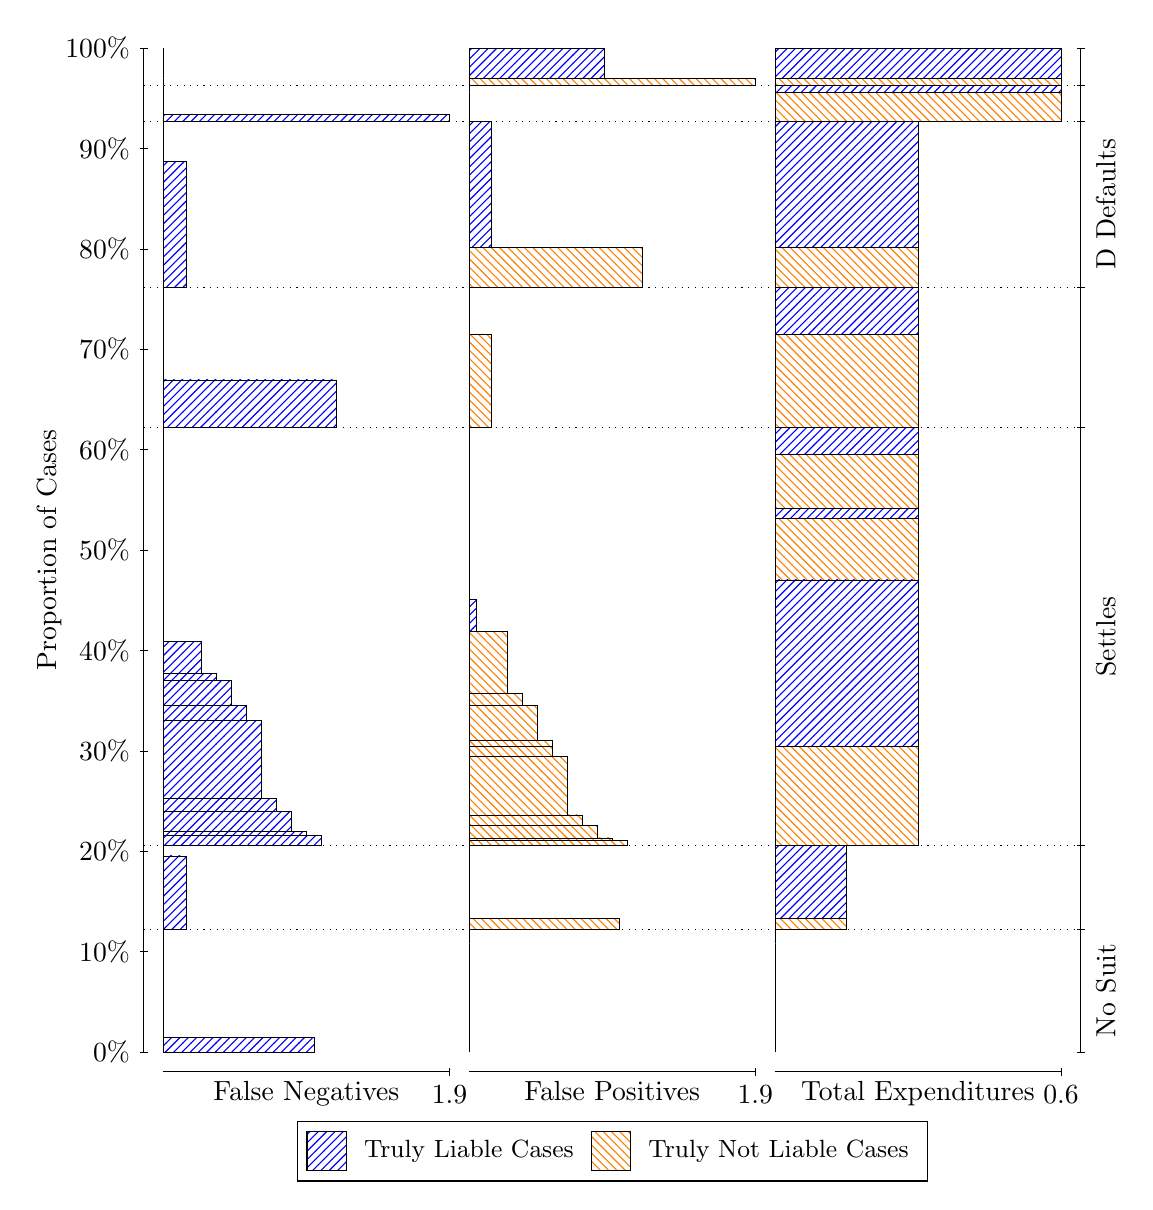
\begin{tikzpicture}
\draw[black, very thin] (1.5,1.75) -- (1.5,14.5);
\node[rotate=90, anchor=center] at (0.3, 8.125) {Proportion of Cases};
\draw[black, very thin] (1.45,1.75) -- (1.55,1.75);
\node[anchor=east] at (1.45, 1.75) {0\%};
\draw[black, very thin] (1.45,3.025) -- (1.55,3.025);
\node[anchor=east] at (1.45, 3.025) {10\%};
\draw[black, very thin] (1.45,4.3) -- (1.55,4.3);
\node[anchor=east] at (1.45, 4.3) {20\%};
\draw[black, very thin] (1.45,5.575) -- (1.55,5.575);
\node[anchor=east] at (1.45, 5.575) {30\%};
\draw[black, very thin] (1.45,6.85) -- (1.55,6.85);
\node[anchor=east] at (1.45, 6.85) {40\%};
\draw[black, very thin] (1.45,8.125) -- (1.55,8.125);
\node[anchor=east] at (1.45, 8.125) {50\%};
\draw[black, very thin] (1.45,9.4) -- (1.55,9.4);
\node[anchor=east] at (1.45, 9.4) {60\%};
\draw[black, very thin] (1.45,10.675) -- (1.55,10.675);
\node[anchor=east] at (1.45, 10.675) {70\%};
\draw[black, very thin] (1.45,11.95) -- (1.55,11.95);
\node[anchor=east] at (1.45, 11.95) {80\%};
\draw[black, very thin] (1.45,13.225) -- (1.55,13.225);
\node[anchor=east] at (1.45, 13.225) {90\%};
\draw[black, very thin] (1.45,14.5) -- (1.55,14.5);
\node[anchor=east] at (1.45, 14.5) {100\%};

\draw[black, very thin] (13.4,1.75) -- (13.4,14.5);
\draw[black, very thin] (13.35,1.75) -- (13.45,1.75);
\node[anchor=west] at (13.35, 1.75) {};
\draw[black, very thin] (13.35,3.3108) -- (13.45,3.3108);
\node[anchor=west] at (13.35, 3.3108) {};
\draw[black, very thin] (13.35,4.3704) -- (13.45,4.3704);
\node[anchor=west] at (13.35, 4.3704) {};
\draw[black, very thin] (13.35,9.6849) -- (13.45,9.6849);
\node[anchor=west] at (13.35, 9.6849) {};
\draw[black, very thin] (13.35,11.464) -- (13.45,11.464);
\node[anchor=west] at (13.35, 11.464) {};
\draw[black, very thin] (13.35,13.565) -- (13.45,13.565);
\node[anchor=west] at (13.35, 13.565) {};
\draw[black, very thin] (13.35,14.026) -- (13.45,14.026);
\node[anchor=west] at (13.35, 14.026) {};
\draw[black, very thin] (13.35,14.5) -- (13.45,14.5);
\node[anchor=west] at (13.35, 14.5) {};

\draw[black, very thin, pattern color=blue, pattern=north east lines] (1.75,1.75) rectangle (3.6623,1.931);
\draw[black, very thin, pattern color=orange, pattern=north west lines] (1.75,1.931) rectangle (1.75,3.3108);
\draw[black, very thin, pattern color=blue, pattern=north east lines] (1.75,3.3108) rectangle (2.0368,4.2393);
\draw[black, very thin, pattern color=orange, pattern=north west lines] (1.75,4.2393) rectangle (1.75,4.3704);
\draw[black, very thin, pattern color=blue, pattern=north east lines] (1.75,4.3704) rectangle (3.7579,4.5011);
\draw[black, very thin, pattern color=blue, pattern=north east lines] (1.75,4.5011) rectangle (3.5667,4.5494);
\draw[black, very thin, pattern color=blue, pattern=north east lines] (1.75,4.5494) rectangle (3.3754,4.8099);
\draw[black, very thin, pattern color=blue, pattern=north east lines] (1.75,4.8099) rectangle (3.1842,4.9659);
\draw[black, very thin, pattern color=blue, pattern=north east lines] (1.75,4.9659) rectangle (2.993,5.9622);
\draw[black, very thin, pattern color=blue, pattern=north east lines] (1.75,5.9622) rectangle (2.8018,6.1549);
\draw[black, very thin, pattern color=blue, pattern=north east lines] (1.75,6.1549) rectangle (2.6105,6.474);
\draw[black, very thin, pattern color=blue, pattern=north east lines] (1.75,6.474) rectangle (2.4193,6.5532);
\draw[black, very thin, pattern color=blue, pattern=north east lines] (1.75,6.5532) rectangle (2.2281,6.9666);
\draw[black, very thin, pattern color=orange, pattern=north west lines] (1.75,6.9666) rectangle (1.75,9.6849);
\draw[black, very thin, pattern color=blue, pattern=north east lines] (1.75,9.6849) rectangle (3.9491,10.285);
\draw[black, very thin, pattern color=orange, pattern=north west lines] (1.75,10.285) rectangle (1.75,11.464);
\draw[black, very thin, pattern color=blue, pattern=north east lines] (1.75,11.464) rectangle (2.0368,13.06);
\draw[black, very thin, pattern color=orange, pattern=north west lines] (1.75,13.06) rectangle (1.75,13.565);
\draw[black, very thin, pattern color=blue, pattern=north east lines] (1.75,13.565) rectangle (5.3833,13.654);
\draw[black, very thin, pattern color=orange, pattern=north west lines] (1.75,13.654) rectangle (1.75,14.026);
\draw[black, very thin, pattern color=orange, pattern=north west lines] (1.75,14.026) rectangle (1.75,14.116);
\draw[black, very thin, pattern color=blue, pattern=north east lines] (1.75,14.116) rectangle (1.75,14.5);
\draw[black, very thin, pattern color=orange, pattern=north west lines] (5.6333,1.75) rectangle (5.6333,3.1299);
\draw[black, very thin, pattern color=blue, pattern=north east lines] (5.6333,3.1299) rectangle (5.6333,3.3108);
\draw[black, very thin, pattern color=orange, pattern=north west lines] (5.6333,3.3108) rectangle (7.5456,3.442);
\draw[black, very thin, pattern color=blue, pattern=north east lines] (5.6333,3.442) rectangle (5.6333,4.3704);
\draw[black, very thin, pattern color=orange, pattern=north west lines] (5.6333,4.3704) rectangle (7.6412,4.4386);
\draw[black, very thin, pattern color=orange, pattern=north west lines] (5.6333,4.4386) rectangle (7.45,4.4687);
\draw[black, very thin, pattern color=orange, pattern=north west lines] (5.6333,4.4687) rectangle (7.2588,4.6288);
\draw[black, very thin, pattern color=orange, pattern=north west lines] (5.6333,4.6288) rectangle (7.0675,4.7616);
\draw[black, very thin, pattern color=orange, pattern=north west lines] (5.6333,4.7616) rectangle (6.8763,5.5069);
\draw[black, very thin, pattern color=orange, pattern=north west lines] (5.6333,5.5069) rectangle (6.6851,5.6285);
\draw[black, very thin, pattern color=orange, pattern=north west lines] (5.6333,5.6285) rectangle (6.6851,5.7035);
\draw[black, very thin, pattern color=orange, pattern=north west lines] (5.6333,5.7035) rectangle (6.4939,6.1555);
\draw[black, very thin, pattern color=orange, pattern=north west lines] (5.6333,6.1555) rectangle (6.3026,6.3075);
\draw[black, very thin, pattern color=orange, pattern=north west lines] (5.6333,6.3075) rectangle (6.1114,7.0888);
\draw[black, very thin, pattern color=blue, pattern=north east lines] (5.6333,7.0888) rectangle (5.7289,7.5021);
\draw[black, very thin, pattern color=blue, pattern=north east lines] (5.6333,7.5021) rectangle (5.6333,9.6849);
\draw[black, very thin, pattern color=orange, pattern=north west lines] (5.6333,9.6849) rectangle (5.9202,10.864);
\draw[black, very thin, pattern color=blue, pattern=north east lines] (5.6333,10.864) rectangle (5.6333,11.464);
\draw[black, very thin, pattern color=orange, pattern=north west lines] (5.6333,11.464) rectangle (7.8325,11.968);
\draw[black, very thin, pattern color=blue, pattern=north east lines] (5.6333,11.968) rectangle (5.9202,13.565);
\draw[black, very thin, pattern color=orange, pattern=north west lines] (5.6333,13.565) rectangle (5.6333,13.937);
\draw[black, very thin, pattern color=blue, pattern=north east lines] (5.6333,13.937) rectangle (5.6333,14.026);
\draw[black, very thin, pattern color=orange, pattern=north west lines] (5.6333,14.026) rectangle (9.2667,14.116);
\draw[black, very thin, pattern color=blue, pattern=north east lines] (5.6333,14.116) rectangle (7.3544,14.5);
\draw[black, very thin, pattern color=orange, pattern=north west lines] (9.5167,1.75) rectangle (9.5167,3.1299);
\draw[black, very thin, pattern color=blue, pattern=north east lines] (9.5167,3.1299) rectangle (9.5167,3.3108);
\draw[black, very thin, pattern color=orange, pattern=north west lines] (9.5167,3.3108) rectangle (10.425,3.442);
\draw[black, very thin, pattern color=blue, pattern=north east lines] (9.5167,3.442) rectangle (10.425,4.3704);
\draw[black, very thin, pattern color=orange, pattern=north west lines] (9.5167,4.3704) rectangle (11.333,5.6285);
\draw[black, very thin, pattern color=blue, pattern=north east lines] (9.5167,5.6285) rectangle (11.333,7.7456);
\draw[black, very thin, pattern color=orange, pattern=north west lines] (9.5167,7.7456) rectangle (11.333,8.5268);
\draw[black, very thin, pattern color=blue, pattern=north east lines] (9.5167,8.5268) rectangle (11.333,8.6575);
\draw[black, very thin, pattern color=orange, pattern=north west lines] (9.5167,8.6575) rectangle (11.333,9.3365);
\draw[black, very thin, pattern color=blue, pattern=north east lines] (9.5167,9.3365) rectangle (11.333,9.6849);
\draw[black, very thin, pattern color=orange, pattern=north west lines] (9.5167,9.6849) rectangle (11.333,10.864);
\draw[black, very thin, pattern color=blue, pattern=north east lines] (9.5167,10.864) rectangle (11.333,11.464);
\draw[black, very thin, pattern color=orange, pattern=north west lines] (9.5167,11.464) rectangle (11.333,11.968);
\draw[black, very thin, pattern color=blue, pattern=north east lines] (9.5167,11.968) rectangle (11.333,13.565);
\draw[black, very thin, pattern color=orange, pattern=north west lines] (9.5167,13.565) rectangle (13.15,13.937);
\draw[black, very thin, pattern color=blue, pattern=north east lines] (9.5167,13.937) rectangle (13.15,14.026);
\draw[black, very thin, pattern color=orange, pattern=north west lines] (9.5167,14.026) rectangle (13.15,14.116);
\draw[black, very thin, pattern color=blue, pattern=north east lines] (9.5167,14.116) rectangle (13.15,14.5);
\draw[black, dotted] (1.5,3.3108) -- (13.4,3.3108);
\draw[black, dotted] (1.5,4.3704) -- (13.4,4.3704);
\draw[black, dotted] (1.5,9.6849) -- (13.4,9.6849);
\draw[black, dotted] (1.5,11.464) -- (13.4,11.464);
\draw[black, dotted] (1.5,13.565) -- (13.4,13.565);
\draw[black, dotted] (1.5,14.026) -- (13.4,14.026);
\draw[black, very thin] (1.75,1.5) -- (5.3833,1.5);
\node[anchor=north] at (3.5667, 1.5) {False Negatives};
\draw[black, very thin] (5.3833,1.45) -- (5.3833,1.55);
\node[anchor=north] at (5.3833, 1.45) {1.9};

\draw[black, very thin] (5.6333,1.5) -- (9.2667,1.5);
\node[anchor=north] at (7.45, 1.5) {False Positives};
\draw[black, very thin] (9.2667,1.45) -- (9.2667,1.55);
\node[anchor=north] at (9.2667, 1.45) {1.9};

\draw[black, very thin] (9.5167,1.5) -- (13.15,1.5);
\node[anchor=north] at (11.333, 1.5) {Total Expenditures};
\draw[black, very thin] (13.15,1.45) -- (13.15,1.55);
\node[anchor=north] at (13.15, 1.45) {0.6};

\node[black, centered, rotate=90] at (13.72, 2.5304) {No Suit};

\node[black, centered, rotate=90] at (13.72, 7.0277) {Settles};

\node[black, centered, rotate=90] at (13.72, 12.514) {D Defaults};



\draw (7.449999999999999,1.5) node[draw=none] (baseCoordinate) {};
\begin{scope}[align=center]
        \matrix[scale=0.5, draw=black, below=0.5cm of baseCoordinate, nodes={draw}, column sep=0.1cm]{
            \node[rectangle, draw, minimum width=0.5cm, minimum height=0.5cm, pattern=north east lines, pattern color=blue] {}; &
            \node[draw=none, font=\small] (B) {Truly Liable Cases}; &
            \node[rectangle, draw, minimum width=0.5cm, minimum height=0.5cm, pattern=north west lines, pattern color=orange] {}; &
            \node[draw=none, font=\small] (B) {Truly Not Liable Cases}; \\
            };
\end{scope}

\end{tikzpicture}
\end{document}